\documentclass{article}

\usepackage[english]{babel}

\usepackage{graphicx}
\usepackage[shortlabels]{enumitem}
\usepackage{amsmath}
\usepackage{amssymb}
\usepackage{multicol}
\usepackage{blkarray}
\usepackage{tikz}
\usepackage[margin=1.0in]{geometry}
\usepackage{hyperref}

\newcommand{\floor}[1]{\left\lfloor#1\right\rfloor}
\newcommand{\ceil}[1]{\left\lceil#1\right\rceil}
\newcommand{\qed}{\hspace{10mm}$\square$}
\newcommand{\spacer}{\\ \linebreak}
\newcommand{\cycl}[1]{\mathcal{#1}}
\newcommand{\lazy}{edge deletions, vertex deletions and edge contractions}
\newcommand{\lazyspc}{edge deletions, vertex deletions and edge contractions }
\newcommand{\st}{\:|\:}
\newcommand{\colorize}[2]{\color{#1}#2\color{black}}

\title{Discrete Structures I \\ Exercises}
\author{Ella Noomen \& Alessandro Biagiotti}
\date{}

\begin{document}
\maketitle
\clearpage{}
\tableofcontents
\section*{First sheet}
\subsection*{Exercise 1} 
\boldmath \textbf{A graph is \textit{connected} if, for any vertices $u, v \in V(G), G$ contains a 
$u - v$ path.\\ 
Prove that a graph or its complement is connected, possibly both.} \vspace{10pt}\\ \unboldmath 
To solve the exercise we will just provide two different proofs, the first one is the following:
\vspace{5pt}\\ \boldmath 
\textbf{$G$ disconnected $\implies$ $G'$ connected}\vspace{5pt}\\ \unboldmath 
If we make the assumption that the graph $G$ is disconnected, then $G$ contains at least two 
connected components.\\ 
If we now build the complementary graph to $G$, $G'$, we will have an edge $\forall v, u : v \in 
V(A) \land u \in V(B)$; where $A$ and $B$ are actually the two connected components we were talking 
about earlier.\\
Since we are saying that we will have an edge between any two pairs of vertices in $V(G)$ then we
are saying that $G'$ is actually connected (the most basic form of connection because we have an
actual edge between every single pair). 
\vspace{2pt}\\\hspace*{3cm}$\square$\vspace*{10pt}\\
\boldmath \textbf{$G$ connected $\implies G'$ connected $\vee\hspace{3pt} G'$
disconnected}\vspace{5pt}\\ \unboldmath 
To prove this second point we will use counterexamples. \\
\begin{center} 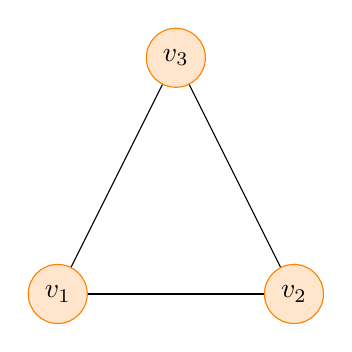
\begin{tikzpicture} \tikzset{% This is the style settings for nodes
        dep/.style={circle,minimum size=0.75cm,fill=orange!20,draw=orange}, c1/.style={-},
        c2/.style={dotted, red, line width=2},
        %c2/.style={orange}, 
        }
        % Nodes
        \node[dep] (n1) at (0,0) {$v_1$}; \node[dep] (n2) at (3,0) {$v_2$}; \node[dep] (n3) at
        (1.5,3) {$v_3$}; 
        %Edges
        \draw[c1] (n1) edge node[above] {} (n2); \draw[c1] (n1) edge node[above] {} (n3); \draw[c1] (n2)
edge node[above] {} (n3); \end{tikzpicture} \hspace*{3cm} \begin{tikzpicture} \tikzset{% This is the
        style settings for nodes dep/.style={circle,minimum size=0.75cm,fill=orange!20,draw=orange},
        c1/.style={-}, c2/.style={dotted, red, line width=2},
        %c2/.style={orange}, 
        }
        % Nodes
        \node[dep] (n1) at (0,0) {$v_1$}; \node[dep] (n2) at (3,0) {$v_2$}; \node[dep] (n3) at
        (1.5,3) {$v_3$}; 
        %Edges
\end{tikzpicture}  \end{center} In the case above we start with a connected graph and we get a
disconnected complementary graph.\vspace{15pt}\\ \begin{center} \begin{tikzpicture} \tikzset{% This
        is the style settings for nodes dep/.style={circle,minimum
        size=0.75cm,fill=orange!20,draw=orange}, c1/.style={-}, c2/.style={dotted, red, line
        width=2},
        %c2/.style={orange}, 
        }
        % Nodes
        \node[dep] (n1) at (0,0) {$v_1$}; \node[dep] (n2) at (3,0) {$v_2$}; \node[dep] (n3) at
        (0,-1.5) {$v_3$}; \node[dep] (n4) at (1.5,-3) {$v_4$}; \node[dep] (n5) at (3,-3) {$v_5$}; 
        %Edges
        \draw[c1] (n1) edge node[above] {} (n3); \draw[c1] (n2) edge node[above] {} (n3); \draw[c1]
        (n3) edge node[above] {} (n4); \draw[c1] (n2) edge node[above] {} (n5); \draw[c1] (n4) edge
        node[above] {} (n2);

\end{tikzpicture}   \hspace*{3cm} \begin{tikzpicture} \tikzset{% This is the style settings for
        nodes dep/.style={circle,minimum size=0.75cm,fill=orange!20,draw=orange}, c1/.style={-},
        c2/.style={dotted, red, line width=2},
        %c2/.style={orange}, 
        }
        % Nodes
        \node[dep] (n1) at (0,0) {$v_1$}; \node[dep] (n2) at (3,0) {$v_2$}; \node[dep] (n3) at
        (0,-1.5) {$v_3$}; \node[dep] (n4) at (1.5,-3) {$v_4$}; \node[dep] (n5) at (3,-3) {$v_5$}; 
        %Edges
        \draw[c1] (n1) edge node[above] {} (n2); \draw[c1] (n1) edge node[above] {} (n4); \draw[c1] (n1)
        edge node[above] {} (n5); \draw[c1] (n3) edge node[above] {} (n5); \draw[c1] (n4) edge node[above]
{} (n5); \end{tikzpicture} \end{center} It is perfectly clear that, while the starting graph is
connected, the complementary is still connected itself.

\subsection*{Exercise 2}
\textbf{Use complete graphs and counting arguments to show the following.}
\begin{enumerate}[a)]
    \item $\binom{n}{2} = \binom{k}{2} + k(n-k) + \binom{n-k}{2} \text{ for } 0 \leq k \leq n $ \\
    \linebreak 
    We know that \begin{equation}\binom{n}{k} = \frac{n!}{k!(n-k)!}\end{equation} \\ 
    Therefore, \\ 
    \linebreak 
    \begin{equation}
        \binom{n}{2} = \frac{n!}{2!(n-2)!} = \frac{n!}{2(n-2)}
    \end{equation}
    \begin{equation}
        \binom{k}{2} = \frac{k!}{2!(k-2)!} = \frac{k!}{2(k-2)}
    \end{equation}
    \begin{equation}
        \binom{n-k}{2} = \frac{(n-k)!}{2!(n-k-2)!} = \frac{(n-k)!}{2(n-k-2)!}
    \end{equation}
    Hence, 
    \begin{align}
    \notag
        \frac{n!}{2(n-2)!} &= \frac{k!}{2(k-2)!} + k(n-k) + \frac{(n-k)!}{2(n-k-2)!} \\
        \notag
        \frac{n(n-1)}{2} &= \frac{k(k-1)}{2} + k(n-k) + \frac{(n-k)(n-k-1)}{2} \\
        \notag
        n(n-1) &= k(k-1) + 2(k(n-k)) + (n-k)(n-k-1) \\
        \notag
        n^2 - n &= k^2 - k + 2nk - 2k^2 + n^2 - nk - n - nk + k^2 + k \\
        n^2 - n &= n^2 - n \hspace{7cm} \square
    \end{align}
    We can also prove the claim using complete graphs. Let $n$ be the number of vertices in a graph $G$. Then, $\binom{n}{2}$ is the cardinality of the edge set of $G$, hence $|E(G)| = \frac{n(n-1)}{2}$. \\
    \linebreak 
    Take a complete graph on $n$ vertices $\mathcal{K}_n$. To make the explanation more apparent we will use an example graph below with $n = 5$ and $k = 3$, note that the meaning of all of the components inside the equation can be generalized.
\begin{enumerate}
    \item $\binom{n}{2}$ is just the number of edges in a complete graph, in our case it amounts to 20.
        \begin{center}
    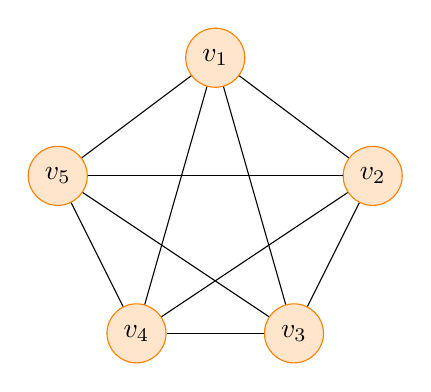
\begin{tikzpicture}
    \tikzset{
    dep/.style={circle,minimum size=0.75cm,fill=orange!20,draw=orange},
    c1/.style={-},
    c2/.style={dotted, red, line width=2},
    }
    \node[dep] (n1) at (3,3) {$v_1$};
    \node[dep] (n2) at (5,1.5) {$v_2$};
    \node[dep] (n3) at (4, -0.5) {$v_3$}; 
    \node[dep] (n4) at (2, -0.5) {$v_4$};
    \node[dep] (n5) at (1, 1.5) {$v_5$};

    \draw[c1] (n1) edge node[above] {} (n2);
    \draw[c1] (n1) edge node[above] {} (n3);
    \draw[c1] (n1) edge node[above] {} (n4);
    \draw[c1] (n1) edge node[above] {} (n5);
    \draw[c1] (n2) edge node[above] {} (n3);
    \draw[c1] (n2) edge node[above] {} (n4);
    \draw[c1] (n2) edge node[above] {} (n5);
    \draw[c1] (n3) edge node[above] {} (n4);
    \draw[c1] (n3) edge node[above] {} (n5);
    \draw[c1] (n4) edge node[above] {} (n5);
\end{tikzpicture}   
\end{center}
    \item $\binom{k}{2}$ is the size of a clique chosen inside the graph of size $k$. We know that this clique must exist for any choice of $k$ vertices, as the graph would otherwise not be complete. This accounts for all of the edges contained inside the clique and nothing more. We will call this subgraph $H$. In our specific case the size of the clique is 3 (in red below).
        \begin{center}
    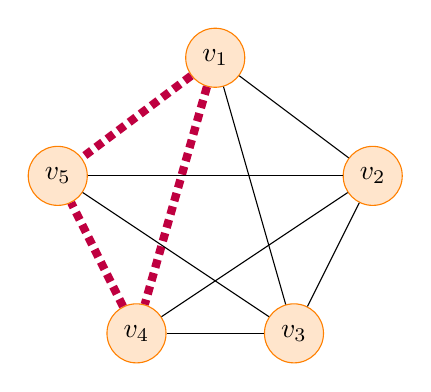
\begin{tikzpicture}
    \tikzset{
    dep/.style={circle,minimum size=0.75cm,fill=orange!20,draw=orange},
    c1/.style={-},
    c2/.style={dotted, purple, line width=3},
    }
    \node[dep] (n1) at (3,3) {$v_1$};
    \node[dep] (n2) at (5,1.5) {$v_2$};
    \node[dep] (n3) at (4, -0.5) {$v_3$}; 
    \node[dep] (n4) at (2, -0.5) {$v_4$};
    \node[dep] (n5) at (1, 1.5) {$v_5$};

    \draw[c1] (n1) edge node[above] {} (n2);
    \draw[c1] (n1) edge node[above] {} (n3);
    \draw[c2] (n1) edge node[above] {} (n4);
    \draw[c2] (n1) edge node[above] {} (n5);
    \draw[c1] (n2) edge node[above] {} (n3);
    \draw[c1] (n2) edge node[above] {} (n4);
    \draw[c1] (n2) edge node[above] {} (n5);
    \draw[c1] (n3) edge node[above] {} (n4);
    \draw[c1] (n3) edge node[above] {} (n5);
    \draw[c2] (n4) edge node[above] {} (n5);

\end{tikzpicture}   
\end{center}
    \item $k(n - k)$ is the amount of edges that link any vertex inside $H$ with any vertex outside of $H$, we will call this second subgraph $H'$. In our specific case the number of edges connecting $H$ and $H'$ is 6 (in green below).
    \begin{center}
    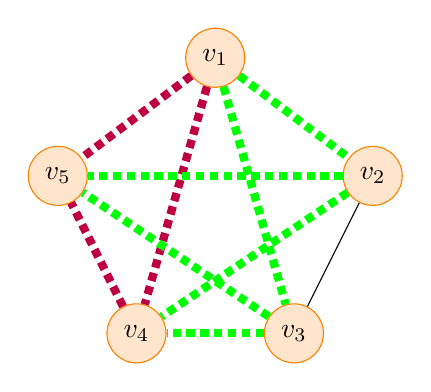
\begin{tikzpicture}
    \tikzset{
    dep/.style={circle,minimum size=0.75cm,fill=orange!20,draw=orange},
    c1/.style={-},
    c2/.style={dotted, purple, line width=3},
    c3/.style={dotted, green, line width=3},
    }
    \node[dep] (n1) at (3,3) {$v_1$};
    \node[dep] (n2) at (5,1.5) {$v_2$};
    \node[dep] (n3) at (4, -0.5) {$v_3$}; 
    \node[dep] (n4) at (2, -0.5) {$v_4$};
    \node[dep] (n5) at (1, 1.5) {$v_5$};

    \draw[c3] (n1) edge node[above] {} (n2);
    \draw[c3] (n1) edge node[above] {} (n3);
    \draw[c2] (n1) edge node[above] {} (n4);
    \draw[c2] (n1) edge node[above] {} (n5);
    \draw[c1] (n2) edge node[above] {} (n3);
    \draw[c3] (n2) edge node[above] {} (n4);
    \draw[c3] (n2) edge node[above] {} (n5);
    \draw[c3] (n3) edge node[above] {} (n4);
    \draw[c3] (n3) edge node[above] {} (n5);
    \draw[c2] (n4) edge node[above] {} (n5);

\end{tikzpicture}   
\end{center}
    \item $\binom{n - k}{2}$ is the amount of edges that connect all of the vertices that are inside $H'$, thus outside of our clique. In our specific case we have just the one show in blue below.
    \begin{center}
    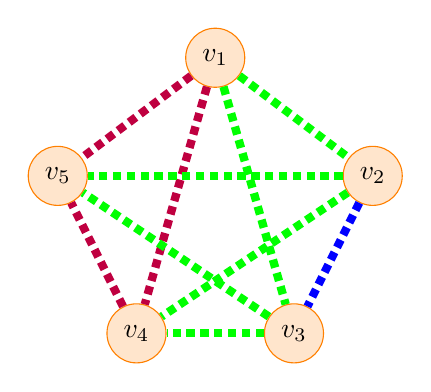
\begin{tikzpicture}
    \tikzset{
    dep/.style={circle,minimum size=0.75cm,fill=orange!20,draw=orange},
    c1/.style={-},
    c2/.style={dotted, purple, line width=3},
    c3/.style={dotted, green, line width=3},
    c4/.style={dotted, blue, line width=3},
    }
    \node[dep] (n1) at (3,3) {$v_1$};
    \node[dep] (n2) at (5,1.5) {$v_2$};
    \node[dep] (n3) at (4, -0.5) {$v_3$}; 
    \node[dep] (n4) at (2, -0.5) {$v_4$};
    \node[dep] (n5) at (1, 1.5) {$v_5$};

    \draw[c3] (n1) edge node[above] {} (n2);
    \draw[c3] (n1) edge node[above] {} (n3);
    \draw[c2] (n1) edge node[above] {} (n4);
    \draw[c2] (n1) edge node[above] {} (n5);
    \draw[c4] (n2) edge node[above] {} (n3);
    \draw[c3] (n2) edge node[above] {} (n4);
    \draw[c3] (n2) edge node[above] {} (n5);
    \draw[c3] (n3) edge node[above] {} (n4);
    \draw[c3] (n3) edge node[above] {} (n5);
    \draw[c2] (n4) edge node[above] {} (n5);

\end{tikzpicture}   
\end{center}
\end{enumerate}
All in all we are saying the following, if we consider a complete graph:
\begin{align*}
    \text{Total number of edges} &= \text{Edges inside a clique of size $k$} \\ &+ \text{Number of edges connecting the clique to the rest of the graph} \\ &+ \text{Edges that connect the nodes that are not in the clique}
\end{align*}
    
    \item If $\Sigma^k_{i=1}n_1 = n \text{ for } 
 n_1, ..., n_k \in \mathbb{N}_0, \text{ then } \Sigma^k_{i=1} \binom{n_i}{2} \leq \binom{n}{2}$ \\
 \linebreak 
 Let \begin{align}
 \notag
 \Sigma^k_{i=1} \binom{n_i}{2} & = \Sigma^k_{i=1} \frac{n_i!}{2!(n_i-2)} \\
 \notag
  & = \frac{1}{2}\Sigma^k_{i=1} n_i(n_i-1) \\
  \notag
  & = \frac{1}{2}(\Sigma^k_{i=1} n_i^2 - \Sigma^k_{i=1} n_i) \\
  & = \frac{1}{2}((\Sigma^k_{i=1} n_i^2) - n)
 \end{align}
and 
\begin{align}
\notag
    \binom{n}{2} & = \frac{n!}{2!(n-2)!} = \frac{1}{2}(n^2-n) 
\end{align}
The claim is then, 
\begin{align}
\notag
    \frac{1}{2}((\Sigma^k_{i=1} n_i^2) - n) &\leq \frac{1}{2}(n^2-n) \\
    \notag
    (\Sigma^k_{i=1} n_i^2 - n) &\leq n^2-n \\
    \notag
    \Sigma^k_{i=1} n_i^2 - n &\leq n^2-n \\
    \notag
    \Sigma^k_{i=1} n_i^2 &\leq n^2 
\end{align}
As $\Sigma^k_{i=1}n_1 = n$, we know that $\Sigma^k_{i=1} n_i^2 \leq n^2$ must hold. $\square$
\end{enumerate}
\section*{Exercise 3}
\boldmath
\textbf{Show that any graph $G$ contains a subgraph of minimun degree at least $\frac{d(G)}{2}$}\vspace{10pt}\\
\unboldmath
A subgraph of $G$ is, by definition, a graph built on top of a subset of the edges of $G$ and a subset of the vertices of $G$.\\
I am not really interested in the structure of the graph I am starting to build upon, if the graph is composed just by vertices and there are no edges I think that picking one random vertex in the mix should do the trick and grant the property.\\
In a broader an more generic scenario I will provide a proof by construction, the idea is the following:\\
We start building a generic $G'$ graph which is a pair built this way:
\begin{enumerate}
    \item $V(G')$ - set of vertices that have nonzero degree.
    \item $E(G')$ - $\emptyset$
\end{enumerate}
Now I will pick the vertex of minimum degree in $G$\footnote{\textbf{Side note}: if $\delta(G) < \floor{\frac{d(G)}{2}}$ I will simply ignore the vertex and pick another one as the "minimum degree node" for $G'$ so that I have enough edges to validate the minimum degree statement. The rest of the construction process stays the same.} and call it $w$ in $G'$, I then add $\floor{\frac{d(G)}{2}}$ edges taken from $G$ to $G'$, the idea is to make sure that $d(w) = \floor{\frac{d(G)}{2}}$.\\
Now, to make sure that $d(w) = \delta(G')$ we want to add enough edges so that each vertex $v \neq w$ has $d(v) \geq \floor{\frac{d(G)}{2}}$, what's important for this constructive step is to make sure that vertex $w$ is left untouched.\\
At the end of the second construction step we will have built a subgraph for $G$ with minimum degree $\delta(G') = \floor{\frac{d(G)}{2}}$.
\vspace{2pt}\\\hspace*{2.5cm}$\square$
\section*{Exercise 4}
\boldmath
\textbf{For any $0 \leq k \leq n$, the Johnson graph $J(n, k)$ is the graph defined as follows. The vertex set of
$J(n, k)$ consists of all $k$-elements subsets of $[n]$. Two vertices of $J(n, k)$ are adjacent if and only
if their intersection has size precisely $k-1$.} 
\begin{enumerate}[a)]
    \item \textbf{Draw $J(5, 3)$, clearly labelling all the vertices.} 
    \unboldmath
    \\
    \linebreak 
    The graph $J(5,3)$ has $\binom{n}{k}$ = $\binom{5}{3}$ = 10 vertices as follows: 
    \begin{multicols}{2}
    $v_1 = \{1, 2, 3\}$ \\
    $v_2 = \{1, 2, 4\}$ \\
    $v_3 = \{1, 2, 5\}$ \\
    $v_4 = \{1, 3, 4\}$ \\
    $v_5 = \{1, 3, 5\}$ \\
    $v_6 = \{1, 4, 5\}$ \\
    $v_7 = \{2, 3, 4\}$ \\
    $v_8 = \{2, 3, 5\}$ \\
    $v_9 = \{2, 4, 5\}$ \\
    $v_{10} = \{3, 4, 5\}$ 
    \end{multicols}
    In order for a pair of vertices $u$ and $v$ to be adjacent, the two vertices must have $k-1 = 2$ elements in common, i.e. $|u \cap v| = 2$. Hence, we obtain the following adjacency matrix:
    \[
\begin{blockarray}{ccccccccccc}
& v_1 & v_2 & v_3 & v_4 & v_5 & v_6 & v_7 & v_8 & v_9 & v_{10}\\
\begin{block}{c(cccccccccc)}
  v_1 & 0 & 1 & 1 & 1 & 1 & 0 & 1 & 1 & 0 & 0 \\
  v_2 & 1 & 0 & 1 & 1 & 0 & 1 & 1 & 0 & 1 & 0 \\
  v_3 & 1 & 1 & 0 & 0 & 1 & 1 & 0 & 1 & 1 & 0 \\
  v_4 & 1 & 1 & 0 & 0 & 1 & 1 & 1 & 0 & 0 & 1 \\
  v_5 & 1 & 0 & 1 & 1 & 0 & 1 & 0 & 1 & 0 & 1 \\
  v_6 & 0 & 1 & 1 & 1 & 1 & 0 & 0 & 0 & 1 & 1 \\
  v_7 & 1 & 1 & 0 & 1 & 0 & 0 & 0 & 1 & 1 & 1 \\
  v_8 & 1 & 0 & 1 & 0 & 1 & 0 & 1 & 0 & 1 & 1 \\
  v_9 & 0 & 1 & 1 & 0 & 0 & 1 & 1 & 1 & 0 & 1 \\
  v_{10} & 0 & 0 & 0 & 1 & 1 & 1 & 1 & 1 & 1 & 0 \\
\end{block}
\end{blockarray}
 \]
This results in the graph $G$, where $|V| = 10$ and $|E| = 30$ : \\
\begin{center}
    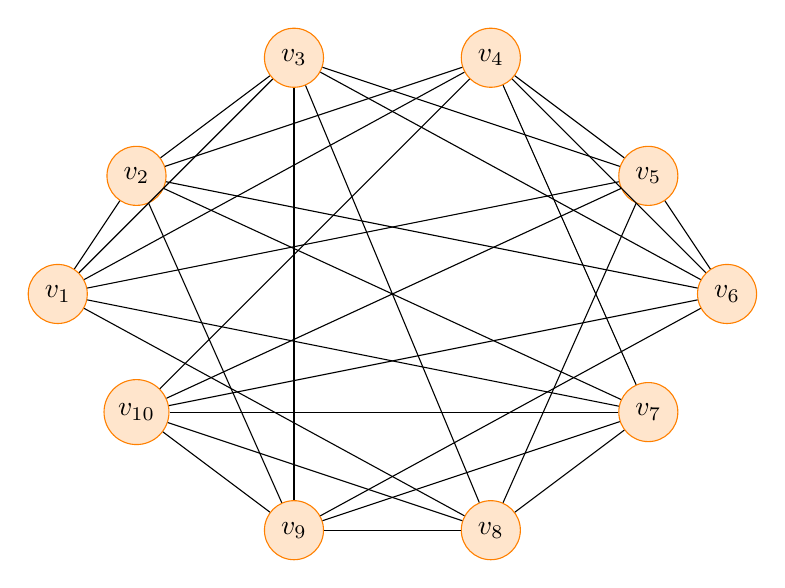
\begin{tikzpicture}
    \tikzset{% This is the style settings for nodes
    dep/.style={circle,minimum size=0.75cm,fill=orange!20,draw=orange},
    c1/.style={-},
    c2/.style={dotted, red, line width=2},
    %c2/.style={orange}, 
    }
    % Nodes
    \node[dep] (n1) at (0,0) {$v_1$};
    \node[dep] (n2) at (1,1.5) {$v_2$};
    \node[dep] (n3) at (3,3) {$v_3$}; 
    \node[dep] (n4) at (5.5,3) {$v_4$};
    \node[dep] (n5) at (7.5,1.5) {$v_5$};
    \node[dep] (n6) at (8.5,0) {$v_6$};
    \node[dep] (n7) at (7.5,-1.5) {$v_7$};
    \node[dep] (n8) at (5.5,-3) {$v_8$};
    \node[dep] (n9) at (3,-3) {$v_9$};
    \node[dep] (n10) at (1,-1.5) {$v_{10}$};
    %Edges
    \draw[c1] (n1) edge node[above] {} (n2);
    \draw[c1] (n1) edge node[above] {} (n3);
    \draw[c1] (n1) edge node[above] {} (n4);
    \draw[c1] (n1) edge node[above] {} (n5);
    \draw[c1] (n1) edge node[above] {} (n7);
    \draw[c1] (n1) edge node[above] {} (n8);
    
    \draw[c1] (n2) edge node[above] {} (n3);
    \draw[c1] (n2) edge node[above] {} (n4);
    \draw[c1] (n2) edge node[above] {} (n6);
    \draw[c1] (n2) edge node[above] {} (n7);
    \draw[c1] (n2) edge node[above] {} (n9);

    \draw[c1] (n3) edge node[above] {} (n5);
    \draw[c1] (n3) edge node[above] {} (n6);
    \draw[c1] (n3) edge node[above] {} (n8);
    \draw[c1] (n3) edge node[above] {} (n9);

    \draw[c1] (n4) edge node[above] {} (n5);
    \draw[c1] (n4) edge node[above] {} (n6);
    \draw[c1] (n4) edge node[above] {} (n7);
    \draw[c1] (n4) edge node[above] {} (n10);

    \draw[c1] (n5) edge node[above] {} (n6);
    \draw[c1] (n5) edge node[above] {} (n8);
    \draw[c1] (n5) edge node[above] {} (n10);

    \draw[c1] (n6) edge node[above] {} (n9);
    \draw[c1] (n6) edge node[above] {} (n10);

    \draw[c1] (n7) edge node[above] {} (n8);
    \draw[c1] (n7) edge node[above] {} (n9);
    \draw[c1] (n7) edge node[above] {} (n10);

    \draw[c1] (n8) edge node[above] {} (n9);
    \draw[c1] (n8) edge node[above] {} (n10);
    
    \draw[c1] (n9) edge node[above] {} (n10);
    
\end{tikzpicture}   
\end{center} 
    \boldmath
    \item \textbf{Show that $J(n, k)$ and $J(n, n-k)$ are isomorphic for any $0 \leq k \leq n.$} \\ 
    \linebreak 
    \unboldmath
    We know that $\binom{n}{k} = \binom{n}{n-k}$ as so $|V|$ will be equal for both. Then, to show the graphs are isomorphic, we must find the isomorphism $\phi$ that preserves the structure of the graph. An isomorphism is just a one to one mapping between two sets. Any binary relation defined on the set is preserved through the isomorphism\footnote{\href{https://www.britannica.com/science/isomorphism-mathematics}{https://www.britannica.com/science/isomorphism-mathematics}}.\\
    \linebreak 
    Let $G_1$ be the graph $J(n,k)$ and $G_2$ the graph $J(n, n-k)$. We know that $\forall v \in V(G_1) \:\: \exists w \in V(G_2) \:\: s.t.\:\: v \cup w = [n]$  and so the bijective mapping is as follows: \\
    \linebreak 
    $\phi : \: \forall v \in V(G_1) \rightarrow w \in V(G_2) \: \text{ where } w = v^c = [n]/v $ \\
    \linebreak
    We now need to prove the function to be bijective, the size of the two sets is the same (because the two binomial coefficients are symmetrical). We now need to prove that there is one to one correspondence between elements of $V(G_1)$ and $V(G_2)$, the process is symmetrical, we will just be proving one direction.\\
    \linebreak
    The idea is actually really simple, let's suppose that $\phi$ is not an isomorphism (thus not a bijection), that means that there is more than one element $w \in V(G_2) \:\: | \:\: \forall v \in V(G_1), \:\: v \cup w = [n]$.
    This means simply that we would have two different elements in $V(G_2)$ representing the same tuple. Since we generate $V(G_2)$ using a binomial coefficient, we are just considering unordered tuples of dimension $k$ that have $|n_1 \cap n_2| < k$ (if the size of the intersection was actually $k$ they would be considered the same tuple), we cannot have two equal tuples inside $V(G_2)$, thus there must be only one tuple in $V(G_2)$ that can be mapped into any element of $V(G_1)$.\\
    \linebreak
    Since we have proven that $\phi$ is a bijection, $\phi$ is actually an isomorphism, which is able to preserve binary relations by definition.
    \boldmath
    \item \textbf{Determine the average degree, number of edges, diameter, and girth of $J(n, k)$ for each
$0 \leq k \leq n$.} \\
\linebreak 
\unboldmath
We know that the number of vertices in a graph $J(n,k) = \binom{n}{k}$. From this we can derive the number of edges: \\
\linebreak 
Two vertices are adjacent iff the length of their intersection = $k-1$, i.e. $\forall u,v \in V(G), uv \in E(G) \text{ if } |u \cap v| = k$, and so there is an edge. We also know that the number of adjacent vertices (neighbours) for each vertex lies in the range $[0, \binom{n}{k}-1]$, and that each vertex will have an equal number of neighbours. Hence, the overall number of edges of the graph lies in the range $[0, \frac{1}{2}\binom{n}{k}(\binom{n}{k}-1)]$.\\  
\linebreak 
First of all, the we know that in a Johnson graph $G$, $d(G) = \delta(G) =\Delta(G)$, in other words, all vertices have the same degree. This is apparent as the sets corresponding to all vertices have the same length, and so by definition must overlap with the same number of vertices/sets. \\
\linebreak 
Now, we must find an exact expression for how many other vertices any given vertex has at least $k-1$ elements in common with (i.e. the intersection has length exactly $k-1$, i.e. they are adjacent). Empirically, we have found that each vertex is adjacent to $k(n-k)$ other vertices. Unfortunately, we are unsure how to prove this formally, but build upon this assumption when calculating the total number of edges.  \\
\linebreak 
As we have $\binom{n}{k}$ vertices, and this expression holds for all vertices, we know that $|E| \leq \binom{n}{k}k(n-k)$. In fact, by the handshaking lemma, we know that each edge has been counted twice in this scenario, and so $|E| = \frac{1}{2}\binom{n}{k}k(n-k)$. \\
\linebreak 
Left to find are the diameter and girth of a Johnson graph. The diameter is colloquially defined as the 'longest shortest' path, i.e. given the set of all distances of all shortest paths between any vertices $u, v \in V(G)$ the diameter is the maximum of all distances. We have again found empirically that the diameter is = $k$ for any graph $J(n, k)$ where $0 \leq k \leq n$. \\
\linebreak 
Finally, the girth of the graph, which is the length of the shortest cycle = 3 (assuming that we have more than 3 vertices). This is the case as the set intersection property is transitive, i.e. for any three vertices $v_1, v_2$ and $v_3$, if $\exists$ edge $v1v2$ and $\exists$ edge $v2v3$, by transitivity there must exist an edge $v1v3$, and so there is a cycle of length 3.

\end{enumerate}

\section*{Exercise 1}
\boldmath
\textbf{Let $G$ be a graph.}
\begin{enumerate}[a)]
    \item \textbf{Prove or disprove: If $u$ and $v$ are the only vertices of odd degree in $G$, then $G$ contains a $u–v$ path.} 
    \unboldmath
    \\
    \linebreak 
    %It should be noted that a cycle is also a path, with the extra condition that for a path $uPv, u=v$ the case that $u = v$, this does not hold.
    %\boldmath
    To prove this we can use the handshaking lemma: ‘The number of vertices of odd degree in a graph is always even.’ (from \textit{Graph Theory} by Reinhardt Diestel, page 5)\\
    \linebreak 
    In the case that $G$ is connected, the statement holds trivially as by definition, $\exists$ a $uv$ path. Hence, we will take a disconnected graph $G$. \\
    \linebreak 
    As the graph is disconnected, $\exists $ at least 2 components of the graph that are not connected. We can use a proof by contradiction to show that $u$ and $v$ must be in the same component, and so $\exists$ a $uv$ path. \\
    \linebreak
    Take $G_1$ and $G_2$ to be two connected components of $G$, where $u \in V(G_1)$ and $v \in V(G_2)$. By the statement, there are no other vertices of odd degree, and so at present both $G_1$ and $G_2$ currently have exactly 1 vertex of odd degree each. \\
    \linebreak 
    As $G_1$ and $G_2$ are graphs in their own right, the handshaking lemma must hold. As $G_1$ and $G_2$ currently both have an odd number of odd degree vertices, the handshaking lemma does not hold, and so we have a contradiction. \\
    \linebreak 
    By this contradiction, $u$ and $v$ must both be in the same component, i.e. $u, v \in V(G_1)$ or $u, v \in V(G_2)$ and so by definition $\exists$ a $uv$ path. Hence, for a graph containing vertices $u$ and $v$ as the only two vertices of odd degree, there must exist a $uv$ path. $\hspace{10mm} \square$ \\
    \linebreak 
    %By the handshaking lemma, this is not possible, as the 
    \boldmath
    \item \textbf{Let $uv \in E(G)$. Prove that $uv$ belongs to at least $d(u)+d(v)-n(G)$ triangles in $G$. (A triangle is a cycle of length 3.)} 
    \unboldmath
    \\
    \linebreak 
    We can prove the statement by induction on the number of vertices in $G$, i.e. $n(G)$. \\
    %Let $t(G, uv)$ denote the number of triangles in $G$ that $uv$ belongs to. \\
    \linebreak 
    Case 1: $n(G) = 2$: $G$ contains only vertices $u$ and $v$ as well as edge $uv$, meaning $d(u) = d(v) = 1$. So, $d(u)+d(v)-n(G) = 1 + 1 - 2 = 0$, which must hold as by definition there are too few vertices to form a cycle of length 3 (or any cycle for that matter). \\
    \linebreak 
    Case 2: $n(G) \geq 3$. Inductive hypothesis: for any graph $G = (V,E)$ with $n(G)$ vertices and an edge $uv \in E(G)$, it holds that the number of triangles sharing the $uv$ edge is $ \geq d(u)+d(v)-n(G)$. \\
    \linebreak
    We must now show that the theorem still holds when any number of edges and vertices are added, i.e. the inductive hypothesis holds for any value of $n(G)$ and $e(G)$. \\
    \linebreak 
    When adding a vertex $w$ to the graph $G$ we can observe exactly one of three different behaviours:
    \begin{enumerate}
        \item $w$ is not adjacent to $u$ or $v$, i.e. $w \notin N_G(u) \wedge w \notin N_G(v)$. This means $d(u)$ and $d(v)$ remain the same while $|V(G)|$ increases by $1$, thus decreasing $d(u)+d(v)-n(G)$ by $1$. This means the statement will still hold, as it is impossible for new triangles to have been formed which include the edge $uv$. Note that it is possible that the number of vertices is greater than $d(u)+d(v)$ and thus the result of $d(u)+d(v)-n(G)$ is negative, but since this is a lower bound this poses no problem. 
        \item $w$ is adjacent to either $u$ or $v$, i.e. $w \in N_G(u) \vee w \in N_G(v)$. This means $|V(G)|$ increases by $1$ and either $d(v)$ or $d(u)$ is increased by one. This means $ d(u)+d(v)-n(G)$ is not changed, which holds true because, as in the case above, it is not possible for any triangles including edge $uv$ to have been added. 
        \item $w$ is adjacent to both $v$ or $w$, i.e. $w \in N_G(u) \wedge w \in N_G(v)$. This means both $d(u)$, $d(v)$ and $n(G)$ increased by $1$, thus $d(u)+d(v)-n(G)$ increases overall by $1$. Hence, a new triangle has been added, which makes sense given we now have edges $uw$, $wv$ and $vu$ and so we have a (new) $u-w-v-u$ path of exactly length 3, which is the definition of triangle.  
    \end{enumerate}
    In conclusion, in any of the three possible cases, the theorem holds, meaning that for a graph $G = (V,E)$ and an edge $uv \in E(G)$, it holds that $uv$ belongs to at least $d(u)+d(v)-n(G)$ triangles. \hspace{10mm}$\square$
\end{enumerate}

\section*{Exercise 2}
\boldmath
\textbf{Let $G$ be a graph with at least two vertices. Prove that G has at least two vertices of the same degree.} \\
\linebreak 
\unboldmath
We can prove this statement using a contradiction. Assume that $G$ has no vertices of the same degree, i.e. all degrees are distinct. Note that the degree of a vertex can be any natural number including 0, i.e. $d(v) \in \mathbb{N}_0 \:\: \forall v \in V(G)$. \\
\linebreak 
Take a graph $G$ with $n$ vertices. In order for there to be $n$ distinct degrees, there must be a set of length $n$ describing the degrees of all vertices in the graph where each value $\in \mathbb{N}_0$. We know that the highest degree vertex has degree $n-1$ (as it cannot be adjacent to itself). In order then, for the set to have length $n$, the set must start at 0.  \\
\linebreak 
So, the degrees can be described in the set $\{0, 1, ..., n-1\}$ where the $ith$ vertex has degree $i$. This can be interpreted as follows: \\
\linebreak 
Vertex $n$ has degree $n-1$ (it is adjacent to all vertices except itself), vertex $n-2$ has degree $n-2$ etc. %\\
%\linebreak 
The final vertex, vertex $n-n$, therefore has degree $n-n = 0$. However, it is a contradiction that there should be a vertex $n$ that is adjacent to \textit{all} vertices, as well as vertex that has no adjacent vertices (i.e. degree of 0). \\
\linebreak 
Therefore, we know that it cannot be that all vertices have a distinct degree, and so there must be at least two vertices of the same degree. \hspace*{10mm} $\square$\\



\subsection*{Exercise 3 }
\textbf{Show that any 2-connected graph contains a cycle.} \\
\linebreak
In order for a graph $G$ to be $k-$connected, it must have at least $k+1$ vertices, i.e. $|V(G)| \geq k+1$. So, $V|G| \geq 3$. \\
\linebreak
As $G$ is connected on with $|V(G)| \geq 3$ vertices, $\exists$ at least one vertex $v$ s.t. $d(v) \geq 2$. Let the neighbourhoud $N(v)$ contain vertices $u$ and $w$. \\
\linebreak 
As $G$ is connected, $\exists$ a path $uPw = \{uv, vw\}$. We also know that as $G$ is 2-connected, we can remove either $uv$ or $vw$ without disconnecting the graph. \\
\linebreak 
So, $\exists$ some path $uP'w$ that does not contain $uv$ or $vw$. \\
\linebreak 
As $uPw$ and $uP'w$ are disjoint, we know $\exists$ a cycle $C = uPw \cup uP'w. \hspace{10mm} \square$
\subsection*{Exercise 4}
\boldmath
\textbf{Show that every tree $T$ has at least $\Delta(T)$ leaves.}\\
\unboldmath
\linebreak
\textbf{Proof}\\
Let's consider a generic tree $T$, let's call $\bar{x}$ the vertex with maximum degree $\Delta(T)$.\\
\linebreak
\textbf{Claim 1}\\
For any tree $T$, given a vertex, it is either a leaf itself or there is a path that links it to one.\\
\linebreak
\textbf{Proof}\\
Let's suppose that some vertices are not linked to leaves.\\
Because of theorem 1.15 it's impossible because the following have to hold:
\begin{itemize}
    \item There must be a unique path between any two nodes $u$ and $v$
    \item The tree $T$ is minimally connected
\end{itemize}
If some of the vertices are not linked to the leaves then there are missing arcs inside the tree that would make it disconnected and thus not a tree. Which is a contradiction because $T$ is actually a tree.\\
\linebreak
Getting back to the main proof, if we consider the sons of $\bar{x}$, each one of them must be a leaf himself or be connected to a leaf because of \textbf{Claim 1}. It's important to note that each son is linked to its own unique leaf. If that weren't true we would have two different paths getting to the same leaf, and that would mean that we would have a cycle, thus making $T$ not a tree.\\
Thus for every son of $\bar{x}$ we have at least one corresponding leaf $\implies$ the number of leaves in a tree is at least $\Delta(T)$\\
\vspace{5pt}\hspace{2cm}$\square$
\section*{Sheet 3}
\subsection*{Exercise 1}
\boldmath 
\textbf{Let $G$ be a graph on $n \geq 3$ vertices with $\delta(G) \geq \frac{n}{2}$. Show that $G$ is
$2$-connected.}
\unboldmath\\
\linebreak
\textbf{Proof}\\
We want to prove the above by contradiction, let's suppose that $\delta(G) \geq \frac{n}{2}$ does
not imply is $2$-connectivity.\\
$2$-connectivity would imply the following:
\begin{itemize}
    \item The graph has at least three nodes (which is true by hypothesis).
    \item $G \setminus \{v\}$, where $v$ is a generic vertex inside the graph, is still connected.
\end{itemize}
Since the graph is not $2$-connected removing a vertex actually compromises connectivity, thus
whenever we remove a vertex from $V(G)$ we get two different components that we'll call $A$ and
$B$.\\
\linebreak
Both components must have $\delta(X) = \floor{\frac{n - 1}{2}}$, where $X$ is the generic component.
That means that in both components there has to be a vertex $v$ such that its degree $d_X(v) =
\floor{\frac{n - 1}{2}}$.
Let's suppose that the above statement was not true and, without loss of generality, let's suppose
that $A$ has $\delta(A) > \floor{\frac{n - 1}{2}}$. Then $\delta(B) < \floor{\frac{n - 1}{2}} <
\frac{n}{2}$ because if $\delta(B) \geq \floor{\frac{n - 1}{2}}$ as well it would mean that there
would be a vertex $u$ in $B$ connected to at least as many vertices as $v$ in $A$ and that would be
against the hypothesis because $A \cap B \neq \emptyset$. Thus the graph would still be connected\\
\linebreak
To conclude, since both $A$ and $B$ have a vertex ($v \in V(A) \land u \in V(B)$) that should be connected to at least
$\floor{\frac{n - 1}{2}}$ other vertices, and $N(v) \cap N(u) = \emptyset$ then we can say that
\begin{equation}
    |N(v)| + |N(u)| = n(G)
\end{equation}
thus
\begin{equation*}
    \floor{\frac{n - 1}{2}} + \floor{\frac{n - 1}{2}} + 2\footnote{The $+2$ comes from the fact that
    the neighbourhood does not account for the node itself} = n + 1
\end{equation*}
And that is a contradiction because the graph contains $n$ vertices.\\
This proves that if a graph has at least three vertices and $\delta(G) \geq \frac{n}{2}$, then it
must be $2$-connected. \hspace{10mm} $\square$

\subsection*{Exercise 2}
\boldmath
\textbf{Let $G$ be a $k$-connected graph. Let $G'$ be obtained from $G$ by adding a new vertex and
connecting it to $k$ vertices of $G$. Show that $G'$ is $k$-connected.\spacer
Proof} \\
\unboldmath
A graph $G$ is $k$-connected, if $|V(G)| \geq k+1$ and $\forall \:\:X \subseteq V(G), \:\:|X| < k, \:\:G - X$ is still connected.\spacer
Let's suppose that $G$ is a graph with $n$ vertices and is $k$-connected, we will build $G'$ starting
from $G$ and adding just one vertex (we will call it $v$) connected to $k$ other vertices.\spacer
Let's suppose, for a contradiction, that after adding $v$, $G'$ would not be $k$-connected anymore. This means that by removing a subset of vertices of size less than $k$ from $V(G')$, $G'$ would not be connected anymore.\footnote{It can be trivially proven that, for $G'$, $n(G') > n(G) > k + 1$}\spacer
If we try to remove the biggest set $X \subseteq V(G')$ possible, thus a set of size $k - 1$ we have two possible choices:
\begin{itemize}
    \item $v \in X \implies \:\:$ we are removing $k - 2$ vertices from the subgraph $G$ (which is $k$-connected by hypothesis), thus the graph is still connected.
    \item $v \notin X \implies \:\:$ we remove $k - 1$ vertices from the subgraph $G$. Since $v$ is connected to $k$ of them, we will always have, after removal, at least one vertex in $V(G)$ linked to what remains of $V(G)$. Moreover, since $G$ is $k$-connected, even if we remove $k - 1$ vertices from it the graph will remain connected.
\end{itemize}
Then we have that, no matter how we choose $X \subseteq V(G')$, $G'$ stays connected,
contradicting the hypothesis that $G'$ would not being connected, proving that $G'$ is $k$-connected. \qed
\subsection*{Exercise 3}
\boldmath 
\textbf{Let $T$ be a tree with no vertex of degree $2$ and $n(T) \geq 2$. Show that $T$ has more leaves than
other vertices.}
\unboldmath 
\\ 
\linebreak 
\textbf{Proof}
We will prove the hypothesis via induction over the subtrees in $T$. The idea is the following.\\ 
\linebreak 
We will call the set of the leaves of the tree $V_l(T)$ and the set of internal nodes in the tree as
$V_i(T)$.\\ 
\linebreak 
In the base case we just have the root with a set of sons that is of at least three vertices, the
property trivially holds.\\
\linebreak
The more interesting case is the recursive one, in which I have a tree of a generic dimension, for
which I suppose that $|V_l(T)| > |V_i(T)|$ holds.\\
If I add a subtree to my current tree, whatever the number of sons, I will just be turning one of
the leaves in the root of the subtree and I will be attatching to it $k$ sons. This can be
translated into the following
\begin{equation}
    |V_l(T)| + k > |V_i(T)| + 1
\end{equation}
If the above weren't true we would be having the following
\begin{itemize}
    \item $k = 1$, which would invalidate the fact that any vertex in the tree must have more than two
    sons.
    \item $|V_l(T)| = |V_i(T)|$, which would invalidate our inductive hypothesis.
\end{itemize}
Thus in the end we have that $|V_l(T)| + k > |V_i(T)| + 1$ and thus our property still holds, thus
we have proven that the number of leaves is always greater than the number of internal vertices for
the tree. \hspace{10mm} $\square$

\subsection*{Exercise 4}
\boldmath
\textbf{Prove or disprove: If $e$ is an edge of a connected graph $G$, then $e$ belongs to some spanning tree
of $G$.\spacer 
Proof}
\unboldmath
%A graph $G$ is connected if there exists a $uv$ path $\forall u, v \in V(G)$. \\
%\linebreak 
%A spanning tree $T$ of $G$ is a subset of edges such that these span all vertices of $G$. It has a tree structure, meaning it is: i) minimally connected, ii) maximally acyclic, iii) $\forall u,v \in V(T) \exists$ a unique $uv$ path iv) \\
%\linebreak 
%Assume that there exists some spanning tree $T$ of $G$ that does not contain $e$. This means that $G - e$ is still connected. \\
%\linebreak 

Let $G'$ be the result of removing $e$ from graph $G$. $G'$ can be either connected or disconnected. \\
\linebreak 
%In both cases, there must exist some spanning tree $T$ of $G$ containing edge $G$. \\
\textbf{Case 1}: $G'$ is disconnected \\
If $G$ disconnects the graph, it means there is no longer a $uv$ path $\forall u,v \in V(G)$, which also means there cannot be a spanning tree of $G$ (as not all vertices are accounted for). This means that $e$ was a so-called \textit{bridge} edge, and by definition is contained in every spanning tree $T$ of $G$. As $e$ is contained in all spanning trees, it is contained in some spanning tree. \\
\linebreak 
\textbf{Case 2}: $G'$ is connected \\
As $G'$ is still connected, we know by definition there exists some spanning tree $T$ not containing the edge $e$. This means there exists a path $P = T + e$. By theorem 1.15, we know trees, and therefore, spanning trees, are maximally acylic. So, adding $e$ to $T$ creates a cycle (which contains $e$), meaning $P$ contains exactly one cycle. \\
\linebreak 
Let $x$ be some edge in the cycle $\cycl{C}$ that is not $e$. We can remove $x$ from the cycle $\cycl{C}$ and be left with a path $Y$ that connects all vertices $u, v \in \cycl{C}$. Although we changed the structure of the spanning tree $T$ the connectivity still holds, thus we have built a different spanning tree $T'$, containing $e$ starting from $T$. \\
\linebreak
That proves the thesis. \qed
%Finally, to show that then, there exists some spanning tree containing $P'$ and so $e$, we must show it is not possible that removing $x$ disconnected the original graph $G$. \\
%\linebreak 
%We can prove this easily using a contradiction. Let's assume that 
%So, we we know that $P$ contains exactly one cycle. 
%G-e$. Removing edge $e$ from $G$, resulting in $G'$, can result in the graph e


\subsection*{Exercise 5}
\section*{Sheet 4}
\subsection*{Exercise 1}
\boldmath
\textbf{Let $G$ be a connected graph with no path of length 4 and no cycle of length 3 as a subgraph. Show that $G$ is bipartite.} \\
\unboldmath
\linebreak 
$G$ is a bipartite graph if it contains two components $A$ and $B$ such that no vertex $a \in V(A)$ and $b \in V(B)$ are adjacent. This means that if vertices have degree greater than 0, its adjacent edges must have endpoints in the other component. \\
\linebreak 
As $G$ is connected, there must $\exists$ a $uv$ path $\forall u, v \in V(G)$. As there exists no path of length 4, $|V(G)|$ must be $\leq 3$. If $G$ has either 1 or 2 vertices it is trivially bipartite. Assume, therefore, that $|V(G)| = 3$. \\
\linebreak 
A connected graph $G$ on 3 edges that does not contain a length cycle, means (at least) one pair of vertices is not adjacent. Therefore, let $V = \{u, v, w\}$ and $E = \{uv, vw\}$. \\
\linebreak 
As $v$ and $w$ are not adjacent, they can be placed in the same component $A$. As both vertices are adjacent to $w$, this must be in component $B$. Hence, we have a bipartition of $G$ such that adjacent vertices are in separate components, and non-adjacent vertices are in the same component. \\
\linebreak
In conclusion, a graph $G$ with no path of length 4 and no cycle of length 3, is bipartite. \qed
\subsection*{Exercise 2}
\boldmath
\textbf{Prove or disprove: A connected graph $G$ is bipartite if and only if for any $uv \in E(G)$ there is no $w \in V(G)$ with $dist_G(u,w) = dist_G(v,w).$} \\
\unboldmath 
\linebreak 
As $G$ is bipartite there exists a bipartition $(A, B)$ s.t. $V(A) \cap V(B) = \emptyset$ and $V(A) + V(B) = V(G).$  Assume $u \in V(A)$ and $v \in V(B)$. The claim asserts that there cannot exist a vertex $w$ in either $V(A)$ or $V(B)$ s.t. $dist_G(u, w) = dist_G(v, w)$. \\
\linebreak 
\boldmath
\textbf{$(\Rightarrow)$ If for any $uv \in E(G)$ there is no $w$ such that $dist_G(u,w) = dist_G(v,w)$, then $G$ is bipartite.} \\
\unboldmath
\linebreak 
Without loss of generality, we can assume for a contradiction, that $\exists$ such a vertex $w \in V(A)$. This means $\exists$ a path $uPw$ and a path $vPw$ of equal length. As $G$ is connected both paths must exist and so have length 
$>$ 1. \\
\linebreak
However, as $u$ and $w$ are $\in A$, any path between them must have an equal length. As $v$ and $w$ are in separate components of the bipartition, any path between them must have odd length. \\
\linebreak 
An even number can never equal an odd number and vice versa, and so $dist_G(u, w)$ can never equal $dist_G(v, w)$ for any $w$. Therefore, no such $w$ can exist.\\
\linebreak 
From this contradiction we know that a connected graph $G$ is bipartite if for any $uv \in E(G)$ there is no $w \in V(G)$ with $dist_G(u,w) = dist_G(v,w)$. \\
\linebreak 
\boldmath
\textbf{$(\Leftarrow)$ $G$ is \textit{only} bipartite if for any $uv \in E(G)$ there is no $w$ such that $dist_G(u,w) = dist_G(v,w)$.}  \\
\unboldmath
\linebreak 
It is sufficient to show that, as no such $w$ exists, the graph cannot contain any odd-length cycles, which is a necessary and sufficient condition for bipartite graphs. \\
\linebreak 
There are two ways in which a cycle of odd length can be created: 
\begin{enumerate}
    \item For any pair of adjacent vertices $u$ and $v$, there exists a third vertex $w$ s.t. $dist(u, w) = d(v, w)$. We have shown that no such vertex exists. 
    \item More generally, if there exists some vertex $w$ such that $uPw$ and $vPw$ both have even length. However, per the definition of a bipartite graph, this can never occur. WLOG, we can assume that $u, w\in V(A)$ and $v \in V(B)$. Any path $uPw$ must have even length, whereas any path $vPw$ must have odd length. Hence, it is not possible that both paths have an even length, and so we cannot create any odd-length cycles in this way either. 
\end{enumerate}
This shows that $G$ can have no odd cycles and is therefore bipartite. Only if some vertex $w$ would exist, we would be able to create an odd cycle. This shows that a connected graph $G$ is bipartite if and only if for any $uv \in E(G)$ there is no $w \in V(G)$ with $dist_G(u,w) = dist_G(v,w).$ \qed
\subsection*{Exercise 3}
\begin{enumerate}[a)]
    \boldmath
    \item \textbf{Show that every graph $G$ contains a spanning bipartite subgraph $H$ with $e(H) \geq \frac{e(G)}{2}$.} \\
    \unboldmath
    \linebreak 
    As $G$ is bipartite, $\exists$ two sets $A$ and $B$ s.t. $V(A) \cap V(B) = \emptyset$ and $V(A) + V(B) = V(G).$ \\
    \linebreak 
    We can use a contradiction to show that a spanning bipartite subgraph $H$ of $G$, if it exists, must contain $\geq \frac{e(G)}{2}$ edges. Assume that $e(H) < \frac{e(G)}{2}$. This means we have removed $> \frac{e(G)}{2}$ edges from $G$ and so, there exists some vertex $v$ s.t. $d_H(v) < \frac{d_G(v)}{2}$. \\
    \linebreak 
    Assuming $v \in A$, this means that $v$ has more neighbours in $A$ than in $B$. By maximality, this cannot hold, and so $\forall v \in G, d_H(v) \geq \frac{d_G(v)}{2}$. \\
    \linebreak 
    We can find $e(H)$ by summing over the degrees: $2e(H) = \Sigma_{v \in H} \: d_H(v) \geq \Sigma_{v \in H} \frac{d_G(v)}{2} = e(G)$. From this we get that $e(H) \geq \frac{e(G)}{2}$. \\
    \linebreak 
    With this degree requirement, we can construct a spanning bipartite subgraph $H$ as follows: 
    \begin{enumerate}
        \item  Partition $G$ arbitrarily into two disjoint sets $A$ and $B$ keeping all edges except edges between vertices that are both $\in A$ or both $\in B$.
        \item If the partition is such that for any vertex $v$, $d_H(v)$, we can move this vertex from $A$ to $B$ or from $B$ to $A$, depending on which set it was initially in. 
    \end{enumerate}
    This algorithm must terminate, as the graph is finite, and as $A \cap B = \emptyset$, we know we have constructed a spanning tree with at least $\frac{e(G)}{2}$ edges.  \qed 
    \item \textbf{Can you improve this bound if G is $2k + 1$-regular for some integer $k \geq 1$?} \\
    \unboldmath
    \linebreak 
    We know that as $G$ is bipartite and $k$-regular, for a bipartition $(A, B)$ of $G$, $|A| = |B| = \frac{1}{2}|V(G)|$. \\
    \linebreak 
    WLOG, $e(G) = (2k+1)\cdot|A| = (2k+1)\cdot\frac{1}{2}\cdot|V(G)|$. We also know that, as $G$ is $2k+1$-regular, $|V(G)| \geq 2k+1+1 = 2k+2$. \\
    \linebreak 
    As $e(H) \geq \frac{1}{2}e(G)$:
    \begin{align}
    \notag
    e(H) &\geq \frac{1}{2}((2k+1)\cdot\frac{1}{2}\cdot|V(G)| \\
    \notag
    & \geq \frac{1}{2}((2k+1)\cdot(\frac{1}{2}\cdot|V(G)|)) \\
    \notag
    & \geq \frac{1}{4}\cdot(2k +1)\cdot|V(G)| \\
    & \geq \frac{1}{4}\cdot(2k +1)\cdot(2k+2) \\
    \notag
    & \geq (k+1)(k+\frac{1}{2})
    \end{align}
    Therefore, if $G$ is $2k+1$-regular, a spanning bipartite subgraph $H$ has at least $(k+1)(k+\frac{1}{2})$ edges. 
    \qed  
\end{enumerate}
\subsection*{Exercise 4}
\textbf{Prove proposition 1.26 from the lectures: \\
\linebreak 
The minor relation $\preccurlyeq$ is a partial order on the set of all finite graphs; that is, $\preccurlyeq$ is reflexive, antisymmetric and transitive.} \\
\linebreak
For a graph $G$ and a graph $H$ such that $H \preccurlyeq G$, it holds that $H$ can be obtained by a series of \lazy. The relation is a partial order: 
\begin{itemize}
    \item \textbf{Reflexive}, i.e, $G \preccurlyeq G$ \\
    \linebreak 
    The set of edge deletions, vertex deletions and edge contractions is not required to be non-empty by definition. Therefore, these sets can be empty, resulting in the graph $G$ itself. This implies $G \preccurlyeq G$. 
    \item \textbf{Transitive}, i.e. if $F \preccurlyeq H \preccurlyeq G \rightarrow F \preccurlyeq G$ \\
    \linebreak 
    Let's call $X$ the set of \lazyspc that take us from F to H, let's call $Y$ the set of \lazyspc that take us from H to G. \\
    \linebreak 
    Since those are two sets of operations we can just say that applying $X \cup Y$ to our starting graph $F$ we will get from $F$ to $G$.
    
    \item \textbf{Antisymmetric}, i.e. if $H \preccurlyeq G$ and $G \preccurlyeq H$ then $H = G$ or more precisely, $\exists$ $f : V(G)\to V(H)$ ($H$ and $G$ are isomorphic). \\
    \linebreak
    Let's call $X$ the set of \lazyspc that take us from $H$ to $G$. Since $G$ is $H$'s minor we can say that 
    \begin{equation}
        |V(H)| > |V(G)| \land |E(H)| > |E(G)|\label{eq:minor}
    \end{equation}
    Since we can only remove vertices or edges when building a minor, the minor will always be smaller than the original graph. Thus if $G$ is $H$'s minor $H$ cannot be $G$'s minor, because if it were it would mean that $|V(G)| > |V(H)| \land |E(G)| > |E(H)|$ but that would contradict \eqref{eq:minor}.\\
    \linebreak 
    Of course that only works when we do not perform any changes on the graph, and thus when we are applying reflexive property.
\end{itemize}
In conclusion, we have shown that the minor relation $\preccurlyeq$ is reflexive, transitive and antisymmetric. \qed
\subsection*{Exercise 5}
\boldmath
\textbf{Let $G$ be a connected graph and let $k \geq 3$. Show that the following are equivalent.}
\unboldmath
\begin{enumerate}[a)]
    \boldmath
    \item \textbf{$G$ contains $K_{1,k}$ as a minor. (The complete bipartite graph $K_{1,k}$ is sometimes called a $k$-star, denoted $S_k$.)}
    \unboldmath

    \boldmath
    \item \textbf{$G$ contains a tree with at least $k$ leaves as a subgraph.}
    \unboldmath

    \boldmath
    \item \textbf{$G$ has a spanning tree with at least $k$ leaves.}
    \unboldmath
\end{enumerate}
We will be proving the above statement like we did for statement 1.15 during lectures.
\subsection*{a) $\implies$ b)}
Let's suppose we have a generic graph $G$ having $K_{1, k}$ for a minor. This type of minors are called \textit{Star minors} and we will call $x$ the vertex at the center of the star. Since the graph is connected by hypothesis we can always build a spanning tree $T$ for $G$ by corollary 1.16.\\
\linebreak
At lecture we defined Algorithm 1 that allows us to build a spanning tree starting from a graph $G$ and a vertex. Since we have proven that the algorithm works and we have proven in a previous sheet that any tree $T$ will have at least $\Delta(T)$ leaves, if we build the spanning tree rooted in $x$ and $x$ is the vertex with highest degree into the spanning tree, then we can say that $T$ has at least $k$ leaves. If $x$ is not the vertex with highest degree in $T$ we can say that there is going to be another vertex, called $y$, such that $d_T(y) > d_T(x) = k$ thus we will have a tree rooted in $x$ with surely more than $k$ leaves.\\
\linebreak
The above proves that if $G$ contains a $K_{1, k}$ minor then there is a tree, in particular the spanning tree, $T$ which is subgraph of $G$ that contains at least $k$ leaves. \qed
\subsection*{b) $\implies$ c)}
By hypothesis we have a graph $G$ containing a tree $T$ with at least $k$ leaves. We know from the second sheet that any tree with at least $k$ leaves must have a vertex $x$ with $k$ sons ($\Delta(T) = |S_T(x)| = k$, where $S_T(\cdot)$ is the set of for vertex $x$ in $T$).\\
\linebreak
Then among all of the possible spanning trees for $G$ we can consider the tree $T'$ that contains $x$ and all of its sons. That spanning tree will have, by the same theorem, at least $k$ leaves. \qed
\subsection*{c) $\implies$ a)}
Let's suppose by contradiction that graph $G$ doesn't have a $K_{1, k}$ minor, that means that there is no way for us, starting from $G$, through \lazyspc to get to a $K_{1, k}$ subgraph.\\
\linebreak
Keeping that in mind, by theorem 1.15, any tree is a tree only if it is minimally connected, we can eliminate any vertex / edge, as long as we start from the leaves and we maintain connectivity in the structure.\\
\linebreak
Since $G$ has a spanning tree $T$ with at least $k$ leaves by hypothesis we know from the second sheet that there is a vertex $x \in V(T)$ such that $x$ has $k$ sons. That means that through \lazyspc we can reduce $T$ to the subgraph containing just $x$ and its direct descendants.\\
This subgraph is actually $K_{1, k}$ and, since the minor relation is transitive, being $T$ a minor of $G$, being $K_{1, k}$ a minor of $T$, $K_{1, k}$ is a minor of $G$.\\
\linebreak
That is absurd because we supposed that $G$ didn't admit $K_{1, k}$ as a minor, thus proving that a graph $G$ having a spanning tree with at least $k$ leaves implies that $G$ admits $K_{1, k}$ as a minor. \qed
\section*{Sheet 5}
\subsection*{Exercise 1}
\boldmath
\textbf{Let $G$ be a graph. A \textit{cycle decomposition} of $G$ is a partition of $E(G)$ into cycles (i.e., a set of edge-disjoint cycles of $G$ covering all the edges of $G$). Show that $G$ has a cycle decomposition if and only if each of its connected components contains an Euler tour}. \\
\unboldmath
\linebreak 
An Euler tour is cycle that uses each edge in the graph exactly once. It is a necessary and sufficient condition that a graph contains an Euler tour if all vertices have even degree. \\
\linebreak 
Therefore, we can show that $G$ has a cycle decomposition if and only if all vertices have even degree. WLOG we can consider each component separately. Let $F$ be a connected component of $G$. \\
\linebreak 
\boldmath
($\Rightarrow$) \unboldmath If $F$ has a cycle decomposition $\Rightarrow$ all vertices $\in F$ have even degree. \\
\linebreak 
As $F$ is connected, there are no isolated vertices (vertices of degree 0). Therefore, $\forall v \in V(F)$, $d_F(v) \geq 1$, meaning it belongs to $\geq 1$ cycles. In order for $v$ to belong to a cycle, it must have exactly 1 incoming and 1 outgoing edge. More generally, it will have 1 incoming and 1 outgoing edge for each cycle that it belongs to. This will always be an even number, and so the degree of each vertex is even. \\
\linebreak
\boldmath
($\Leftarrow$) \unboldmath If all vertices in $F$ have even degree $\Rightarrow$ $F$ has a cycle decomposition. We can prove this using induction on $e(F)$. \\
\linebreak 
\textbf{Base case:} In the general case, the base case would be $e(F) = 0$ (as there are no edges, all vertices have degree 0, which is even, and so the graph has a cycle decomposition, which is an empty set). As $F$ is connected, the base case will never occur and we can skip to the inductive step. \\
\linebreak 
\textbf{Inductive hypothesis}: Suppose that $F$ has $< e(F)$ edges. There will exist a cycle decomposition. We can use this to shown that any graph $F$ with $e(F)$ edges has a cycle decomposition. \\
\linebreak 
As all vertices have even degree, there exists at least 1 cycle $C$. We can remove the edges of this cycle from $F$, and so our remaining graph is $F \setminus E(C)$. $F \setminus E(C)$ will have the same vertex set, and since we are removing an even number of edges, the resulting graph will also have only even degree vertices. \\
\linebreak 
We can continue to remove the cycles, each time adding $C$ to a set $\mathcal{C}$. Eventually we will have a graph on $n(F)$ vertices and 0 edges and we have shown that the graph has cycle decomposition $\mathcal{C}$.
\\
\linebreak 
We have shown that the statement holds for any connected component, and will therefore hold for all connected components. $G$ has a cycle decomposition if and only if each of its connected components contains an Euler tour. \qed
\subsection*{Exercise 2}
\begin{enumerate}[a)]
\boldmath
\item \textbf{Prove or disprove: a tree contains at most one perfect matching.} \\
\unboldmath
\linebreak 
\textbf{Proof}\\
We can show that this claim holds for any tree $T$. \\
\linebreak 
A matching $M$ of a graph $G$ is an independent edge set of $G$, meaning that no edge $e \in E(M)$ shares common vertices. A matching $M$ is perfect if $V(M) = V(G)$ (i.e. every vertex is accounted for exactly once). \\
\linebreak For a graph $G = (V, E)$, a perfect matching has size $\frac{|V(G)|}{2}$ and so in order for a graph to have a perfect matching it must have an even number of vertices.  \\
\linebreak 
\textbf{Case 1:} $T$ has an odd number of vertices. This means it cannot have a perfect matching and the claim holds. \\
\linebreak 
\textbf{Case 2}: $T$ has an even number of vertices. Assume, for a contradiction, that there exist two distinct perfect matchings $M_1$ and $M_2$ of $T$. We can show that these matchings are in fact the same.\\
\linebreak
Let $G$ be the graph of $M_1 \cup M_2$. As $M_1$ and $M_2$ are believed to be distinct, $\exists$ some edge $e \in E(G)$ that is $\in E(M_1)$ but $\notin E(M_2)$. This means there is some vertex $v$ of degree $\geq 2$. \\
\linebreak 
However, two distinct perfect matchings that share a vertex would have to alternate between edges $\in T$. This would eventually have to close a cycle in the graph. By definition, trees are acyclic, and so we know that $M_1$ and $M_2$ would have to be the same. \\
\linebreak 
In conclusion, we have shown that a tree $T$ contains at most one perfect matching. \qed
\boldmath 
\item \textbf{Let $G$ be a graph and suppose that $E(G)$ can be partitioned into two matchings. Show that $E(G)$ can be partitioned into two matchings whose sizes differ by at most one.} \\
\unboldmath
\linebreak 
\textbf{Proof}\\
As $E(G)$ can be split into two matchings, $\forall e \in E(G)$, $e \in M_1 \lor e \in M_2$ and $M_1 \cap M_2 = \emptyset$ (otherwise it is not a valid partitioning of the set $E(G)$). It also holds that every vertex has a maximum degree of 2, otherwise $E(G)$ cannot be split into exactly 2 matchings.\\
\linebreak
Suppose, for a contradiction, that $E(G)$ can be split into two matchings $M_1$ and $M_2$ where the sizes of the matchings differ by strictly more than 1. WLOG we can say that $|M_1| \geq |M_2| + 2$ if we say that $|M_2| = x$ then  $|M_1| \geq x + 2$. \\
\linebreak 
In order for both to be valid matchings, for any pair of edges that share a common vertex, one edge must belong to $M_1$ and the other to $M_2$ (otherwise they are not independent sets). \\
\linebreak 
Since $M_1$ is larger than $M_2$ there must be at least one edge $xy \in M_2$ that should actually be in $M_1$.\\
\linebreak
Thus in our case we will have that $M_1$ and $M_2$ have $x$ extremes in common and then we need to have at least two more edges that are incident to some other vertex. At this point, if the graph is disconnected and we have more than one component (disconnected from the main body of the graph) containing two vertices linked by one single edge in $M_2$, then the statement holds true, because we can move edges from $M_2$ to $M_1$ to even the balance. On the other hand, if we consider a generic connected graph, then we would be in the situation where an edge of matching $M_2$ insists on a vertex that is already extreme of some other edge in $M_2$, violating the definition of matching and making the statement absurd.\\
This proves that, if we can partition the edge set with two matchings, the sizes of said matchings should differ for at most one edge. \qed
\end{enumerate}
\subsection*{Exercise 3}
\boldmath
\textbf{Let $G$ be a graph. An independent set of $G$ is a set of pairwise non-adjacent vertices in $G$. Show
that $S \subseteq V(G)$ is an independent set of $G$ if and only if $V (G) \setminus S$ is a vertex cover of $G.$} \\
\unboldmath
\linebreak
For a graph $G = (V, E)$, a vertex cover $U \subseteq V(G)$ s.t. $\forall \: uv \in E(G)$, $u \in U \lor v \in U$. \\
\linebreak 
An independent set $S$ of $G$ is a set of pairwise non-adjacent vertices in $G$, meaning that 
for any pair of vertices $u, v \in V(G)$ if $uv \in E(G)$ then $u \in S \lor v \in S$. Similarly, $\forall uv \in E(G)$ if $u \in S \rightarrow v \notin S$. \\
\linebreak 
We are proving the statement: $S \subseteq V(G)$ is an independent set $\Leftrightarrow V(G) \setminus S$ is a vertex cover. \\
\linebreak 
\textbf{Proof} \\
\linebreak
($\Rightarrow$) If $S \subseteq V(G)$ is an independent set $\Rightarrow V(G) \setminus S$ is a vertex cover. \\
\linebreak 
As $S$ is an independent set, for any pair of adjacent vertices $u, v \in G$, either $u$ or $v$ are $\in S$. For each pair of vertices, assume $u \in S$, then the $"v"$ vertex is in the set of vertices. i.e. in the set of vertices denoted $V(G) \setminus S$. We also know that this is a valid vertex cover as for each set of edges, exactly 1 endpoint is in $V(G) \setminus S$.  \\
\linebreak 
($\Leftarrow$) If $V(G) \setminus S$ is a vertex cover $\Rightarrow S \subseteq V(G)$ is an independent set \\
\linebreak 
As $V(G) \setminus S$ is a vertex cover, there can be no adjacent pairs of vertices in $S$. This would mean that there are vertices that are not accounted for in the vertex cover. Therefore, $S$ is an independent set. \\
\linebreak 
In proving the two statements above, we have shown that $S \subseteq V(G)$ is an independent set of $G$ if and only if $V (G) \setminus S$ is a vertex cover of $G.$
\qed 

\subsection*{Exercise 4}
\begin{enumerate}[a)]
\boldmath
    \item \textbf{Use König’s Theorem (Theorem 2.2) to show that every bipartite graph G has a matching of size at least $\frac{e(G)}{\Delta G}$.}
    \unboldmath \\
    \linebreak
    König's theorem states that for a bipartite graph $G$, the maximum size of a matching equals the minimum size of a vertex cover. \\
    \linebreak 
    \textbf{Proof}\\
    Let's suppose for a contradiction that there only exist matchings $M$ with $|M| < \frac{e(G)}{\Delta(G)}$. This means that, however we picked the matching $M$ for graph $G$, its size will always be less than $\frac{e(G)}{\Delta(G)}$. That means that the maximum matching on $G$ will have to be $< \frac{e(G)}{\Delta(G)}$ as well.
    By König's theorem, this means the size of the minimum vertex cover $U$ is also $< \frac{e(G)}{\Delta(G)}$. \\
    \linebreak
    The inequality $|U| < \frac{e(G)}{\Delta(G)}$ can be rewritten as $|U|\Delta(G) < e(G)$. We can show that this cannot hold. A graph with max degree $\Delta(G)$ needs at least $\Delta(G)+1$ vertices and $\Delta(G)$ edges. \\
    \linebreak 
    Take a graph $G$ with $n(G) = \Delta(G)+1$ vertices and $e(G) = \Delta(G)$. Let $A$ = $\{v\}$ with $v$ being the vertex of maximum degree and $B$ consists of the remaining vertices. Note there are no edges between vertices in $B$ as then $(A, B)$ would not be a valid bipartition. \\
    \linebreak 
    In this minimum case, the minimum vertex cover would have to contain the vertex of maximum degree $v$. However, even in this minimal case, the condition is violated, as we assume: 
    \begin{align}
    \notag
        |U| & \Delta(G) < e(G)\\
        \notag
        \text{ but } 1 \cdot & \Delta(G) \nless \Delta(G)+1 
    \end{align}
    Therefore, we have reached a contradiction. This means the minimum vertex cover, and so the maximal matching has size $\geq \frac{e(G)}{\Delta(G)}$. \qed
    \boldmath
    \item \textbf{Deduce that every subgraph of $K_{n,n}$ with more than $(k-1)n$ edges has a matching of size at least $k$}
    \unboldmath \\
    \linebreak
    \textbf{Proof} \\
    Let $K_{n, n}$ denote a complete bipartite graph with bipartition $(A, B)$, where $|A| = |B| = n$. As $G$ is a complete bipartite graph, with $|A| = |B|$, it must be $k$-regular and so $\delta(G) = \Delta(G) = d(G) = n$. We can use the finding from part a) to prove the statement:
    \begin{align*}
        |M| &\geq \frac{e(G)}{\Delta(G)} &&\text{Because of what we showed earlier}\\
            & > \frac{(k - 1) \cdot n}{\Delta(G)} &&\text{By hypothesis on the number of edges in the matching}\\
            & > \frac{(k - 1) \cdot n}{n}\\
            & > k - 1 \\
            & \geq k
    \end{align*}
    Using the finding from part a), we have been able to show that any subgraph of $K_{n,n}$ with more than $(k-1)\cdot n$ edges has a matching $M$ where $|M| \geq k$. \qed
\end{enumerate}
\subsection*{Exercise 5}
\boldmath
\textbf{Let $G$ be a bipartite graph with bipartition $(A, B)$. Suppose that $|N_G(S)| > |S|$ for all non-empty
$S \subsetneq A$. Prove that every edge of $G$ belongs to a matching of $A$.} \\
\unboldmath
\linebreak
Given a graph $G$ and a subset $A \subseteq V(G)$, a matching of $A$ in $G$ is a matching $M$ such that $\forall a \in A$ is incident to an edge in M. \\
\linebreak 
Furthermore, Hall's theorem states that there exists a matching of $A$ if and only if $|N_G(S)| \geq |S| \:\: \forall \:\: S \subseteq A$. \\
\linebreak 
\textbf{Proof} \\
We must show that for every edge $e \in E(G)$, it is possible to construct a matching using $e$ such that all vertices in $A$ are matched. In general, it does not hold, but the additional condition $|N_G(S)| > |S|$ makes it true. \\
\linebreak 
Take two vertices $a, b \in V(G)$ and its edge $ab \in E(G)$. $ab$ will be the first edge of our matching. Then, all vertices in the set $V(A - \{a\})$ must also be matched, and we know that $|N_G(A-\{a\})| > |A-\{a\}|$ i.e. $ > |A| - 1$ $\geq A$. \\
\linebreak 
We know that it is possible to match all vertices in $V(A - \{a\})$ as Hall's condition for a matching of $(A - \{a\})$ holds: $|N_G(A-\{a\})| \geq |A|$ (as it will also hold for any subset of $V(A-\{a\})$ by the statement). \\
\linebreak 
We have shown that for any choice of $e$, we can construct a matching of $A$ using this edge. So for a bipartite graph $G$ with bipartition $(A, B)$ with the property $|N_G(S)| > |S|$ for all non-empty
$S \subsetneq A$, we can construct a matching of $A$ using any edge in $E(G)$. \qed
\subsection*{Exercise 6}
\boldmath
\textbf{Let $G$ be a bipartite graph with bipartition $(A, B)$, where $|A| \leq |B|$. Suppose that each $a \in A$ satisfies $d_G(a) \geq \frac{|B|}{2}$ and each $b \in B$ satisfies $d_G(b) \geq |A|- \frac{|B|}{2}$. Show that $G$ has a matching of $A$.}
\unboldmath\\
\linebreak
\textbf{Proof}\\
Let's suppose for a contradiction that the graph $G$ does not admit a matching $M$ of $A$. We will call this matching $M_A$. \\
\linebreak 
Since there is no matching for $A$ we know that there is at least 1 vertex $a \in A$ that is unmatched. In general, for any such $a$, one of the following scenarios holds:
\begin{enumerate}
    \item $a$ has no adjacent vertices $\in B$. Assume that this is not the case as this would void the hypothesis, as $a$ will always be unmatched. Therefore, we consider only the case below:
    \item $a$ has no 'free' neighbouring vertices $\in B$. This means that adding one of the adjacent vertices of $a$ would violate the matching as it would no longer be independent. 
\end{enumerate}
Therefore, we will consider the second case, and show how we can remedy this, so that there is indeed a matching of $A$. Take the unmatched vertex $a$. We can find an augmenting path that will 'free up' a vertex $\in N(a)$. The idea is the following: \\
\linebreak 
Let $x$ be a vertex $\in N(a)$. As $x$ is a matched vertex, we know there exist some vertex $a' \in A$ s.t. $xa'$ is an edge $\in M_A$. So, there are two edges $ax$ and $xa'$. We will add $ax$ to $M_A$ and remove $xa'$ from $M_A$. We would then have to find a free neighbour for $a'$ in order for it to be matched. \\
\linebreak 
If this neighbour exists, let's call it $y$, then we have undergone the following procedure: add $ax$ to $M_A$, remove $xa'$ from $M_A$, add $a'y$ to $M_A$. This way, both $a$ and $a'$ are now matched.\\
\linebreak 
If there is no free neighbour for $a'$, we will have to recursively apply to search until we find a vertex with a free neighbour. If we never find such a free vertex, there is simply no matching of $A$. \\
\linebreak 
However, in this particular case we can be sure that the augmenting path search will converge due to the fact that each $a \in A$ satisfies $d_G(a) \geq \frac{|B|}{2}$ and each $b \in B$ satisfies $d_G(b) \geq |A| - \frac{|B|}{2}$, and our matching requires exactly $|A|$ edges. \\
\linebreak 
Therefore, we have reached a contradiction for the statement that the matching $M_A$ cannot exist. In conclusion, we see that a bipartite with degree requirements as stated in the proposition will have a matching of $A$. \qed
\section*{Sheet 6}
\subsection*{Exercise 1}
\begin{enumerate}[a)]
    \boldmath
    \item \textbf{For each $n \in N$ such that $n \geq 3$, give an easy example of a graph on n vertices where the smallest cardinality of a vertex cover is strictly greater than the maximum cardinality of a matching. Justify your answer.}
    \unboldmath
    \begin{figure}[h]
        \centering
        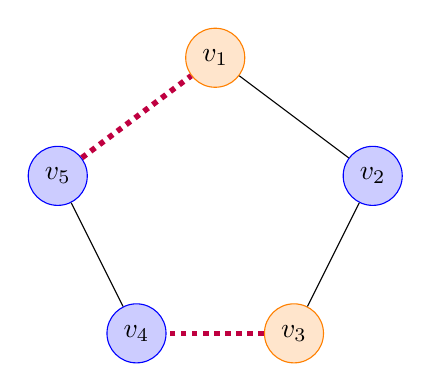
\begin{tikzpicture}
        \tikzset{
        dep/.style={circle,minimum size=0.75cm,fill=orange!20,draw=orange},
        vc/.style={circle, minimum
        size=0.75cm, fill=blue!20, draw=blue},
        c1/.style={-},
        c2/.style={dotted, purple, line width=2},
        }
        \node[dep] (n1) at (3,3) {$v_1$};
        \node[vc] (n2) at (5,1.5) {$v_2$};
        \node[dep] (n3) at (4, -0.5) {$v_3$}; 
        \node[vc] (n4) at (2, -0.5) {$v_4$};
        \node[vc] (n5) at (1, 1.5) {$v_5$}; 

        \draw[c1] (n1) edge node[above] {} (n2);
        \draw[c1] (n2) edge node[above] {} (n3);
        \draw[c2] (n3) edge node[above] {} (n4);
        \draw[c1] (n4) edge node[above] {} (n5);
        \draw[c2] (n5) edge node[above] {} (n1);
        \end{tikzpicture}
        \caption{The minimum vertex cover in \colorize{blue}{\textbf{blue}}, the maximum matching in \colorize {purple}{\textbf{purple}}}
    \end{figure}
    \\
    \linebreak
    \textbf{Justification}\\
    Any graph that is not isomorphic to a bipartite graph must contain a cycle of odd length. \\
    \linebreak
    If the graph $G$ contains a cycle of odd length, our vertex cover will just need $|U_G| = \ceil{\frac{n}{2}} + k$, where $U_G$ is the minimum vertex cover for the graph $G$, $n$ is the length of the cycle and $k$ is a constant value that accounts for the existence of other structures inside the graph that we are not caring for, at the moment.\\
    The above can be explained simply: since every vertex in the cycle has degree 2 then $\ceil{\frac{n}{2}} \cdot 2 > n$.\\
    \linebreak
    If we want to find the corresponding maximum matching we will have to build a walk like the one proposed below:
    \begin{center}
        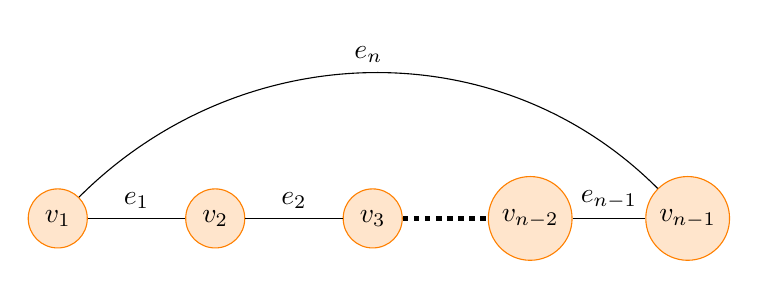
\begin{tikzpicture}
        \tikzset{
        dep/.style={circle,minimum size=0.75cm,fill=orange!20,draw=orange},
        vc/.style={circle, minimum
        size=0.75cm, fill=blue!20, draw=blue},
        c1/.style={-},
        c2/.style={dotted, purple, line width=2},
        c3/.style={dotted, black, line width=2},
        c4/.style={-, out=135, in=45}
        }
        \node[dep] (n1) at (-3,0) {$v_1$};
        \node[dep] (n2) at (-1,0) {$v_2$};
        \node[dep] (n3) at (1,0) {$v_3$}; 
        \node[dep] (n4) at (3,0) {$v_{n - 2}$};
        \node[dep] (n5) at (5,0) {$v_{n - 1}$}; 

        \draw[c1] (n1) edge node[above] {$e_1$} (n2);
        \draw[c1] (n2) edge node[above] {$e_2$} (n3);
        \draw[c3] (n3) edge node[above] {} (n4);
        \draw[c1] (n4) edge node[above] {$e_{n - 1}$} (n5);
        \draw[c4] (n5) edge node[above] {$e_n$} (n1);
        \end{tikzpicture}
    \end{center}
    We will consider the cycle $w = v_1e_1v_2 \dots v_{n - 2}e_{n - 1}v_{n - 1}e_nv_1$.\\
    \linebreak
    Since we are looking for the maximum matching $M$ we will look to add as many edges as possible to the set. Thus we will be alternating edges that are not in $M$ to edges that are in $M$. That translates into taking half of the edges in the cycle ($\frac{n}{2}$). Since, by hypothesis, we know that $n$ is odd then $n - 1$ is even. We can choose two different courses of action:
    \begin{itemize}
        \item $e_1 \in M$, then, by exclusion $e_n \notin M$
        \item $e_1 \notin M$, then, by exclusion $e_n \in M$
    \end{itemize}
    Overall, $|M| = \frac{n - 1}{2} = \floor{\frac{n}{2}}$, but
    \begin{equation}
        \floor{\frac{n}{2}} \leq \ceil{\frac{n}{2}} \label{eq:fundamental}
    \end{equation}
    In the specific case of the odd cycle we can actually say that the floor is strictly less than the ceiling $\implies$ that we will always have a maximum matching which is smaller than the minimum vertex cover.
    \boldmath
    \item \textbf{For each $m, n \in N$ such that $2 \leq m < n$, give an easy example of a graph G on n vertices and $A \subseteq V (G)$ of size m such that G has a matching of A but Hall’s condition does not hold. Justify your answer. (Recall that for a set S of vertices we defined $N(S) := \bigcup_{s\in S} N(s) \setminus S$)} \\
    \linebreak 
    \unboldmath
    As an example, let $m = 1$ and $n = 4$. This satisfies $2 \leq m < n$. In the graph below $A = \{v_4\}$. 
    \begin{figure}[h]
        \centering
        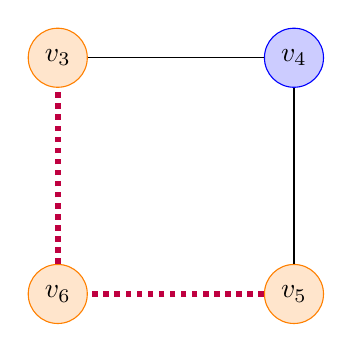
\begin{tikzpicture}
        \tikzset{
        dep/.style={circle,minimum size=0.75cm,fill=orange!20,draw=orange},
        vc/.style={circle, minimum
        size=0.75cm, fill=blue!20, draw=blue},
        c1/.style={-},
        c2/.style={dotted, purple, line width=2},
        c3/.style={dotted, black, line width=2},
        c4/.style={-, out=135, in=45}
        }
        \node[dep] (n3) at (3,1.5) {$v_3$}; 
        \node[vc] (n4) at (6,1.5) {$v_4$};
        \node[dep] (n5) at (6,-1.5) {$v_5$}; 
        \node[dep] (n6) at (3,-1.5) {$v_6$}; 
        
        \draw[c1] (n3) edge node[above] {} (n4);
        \draw[c1] (n4) edge node[above] {} (n5);
        \draw[c2] (n5) edge node[above] {} (n6);
        \draw[c2] (n6) edge node[above] {} (n3);
        \end{tikzpicture}
        \caption{vertices that belong to $A$ are in \colorize{blue}{\textbf{blue}}, the matching is in \colorize{purple}{\textbf{purple}}}
        \label{ex2}
    \end{figure}
    \\\linebreak
    \textbf{Justification}\\
    Let's suppose we have a graph $G$ that is not bipartite\footnote{We consider a non bipartite graph because Hall's condition is a necessary and sufficient condition for a bipartite graph to have an A-perfect matching}, we pick a generic $A \subseteq V(G)$ and we are looking for an A-perfect matching $M_A$, we also suppose Hall's condition doesn't hold, which means that $|N_G(A)| < |A|$.\\
    The only way for a matching to be formed without having $|N_G(A)| \geq |A|$ is that not all vertices have at least a neighbour outside of $A$.\\
    \linebreak
    If all of the vertices in $A$ have a neighbour that can be used to build $M_A$ but not all of the neighbours are $\notin A$ then we can define Kronecker's delta this way:
    \[
    \delta(v) =
    \begin{cases}
        0, & \text{if } v \in A \\
        1, & \text{if } v \notin A
    \end{cases}
    \]
    Now that we have defined the function we can conclude that, because of how we defined the neighbourhood relation over set of vertices:
    \begin{equation}
        N_G(A) = \bigcup_{v \in A} N_G(v) \setminus A = \sum_{v \in A} \delta(v) \leq |A|
    \end{equation}
    
    
\end{enumerate}
\textbf{(Remark: this shows that the “bipartite”condition in König’s and Hall’s theorems is necessary.)}

\subsection*{Exercise 2}

\boldmath
\textbf{Let $G$ be a graph with no isolated vertex (that is, no vertex of degree 0). An edge cover of $G$ is a set $L$ of edges such that each vertex of $G$ is incident to an edge in $L$.}
\unboldmath

\begin{enumerate}[a)]
    \boldmath
    \item \textbf{Let $M$ be a maximum matching of $G$. Use $M$ to construct an edge cover of $G$ of size $n(G)-|M|$.} \\
    \unboldmath
    \linebreak 
    As $M$ is maximum we know that $\forall v \in V(G)$, either $v$ is matched by an edge in $M$ or it is adjacent to another vertex $v'$ that is matched by an edge in $M$. \\
    \linebreak 
    We can construct the edge cover $L$ starting from the matching $M$. This means that to start $L = M$. If all vertices are accounted for, then we can stop. (In this case, the matching is a perfect matching using exactly $n/2$ edges, and so $|M| = |L|$ and $|M| + |L| = n(G)$.)\\
    \linebreak 
    If this is not the case we must extend the edge cover to account for all vertices. This can be done by iteratively applying the following steps: identify an uncovered vertex $v$ and add any adjacent vertex $v'$ (which will be matched by an edge in $M$ by definition) and add edge $vv'$ to $L$. \\
    \linebreak
    By this method, we are adding as many edges to $L$ as vertices not matched in $M$, which is equal to $n(G) - 2|M|$. In total, therefore, $|L| = |M| + (n(G) - 2|M|) = n(G) - |M|$ edges. 
    \boldmath
    \item \textbf{Let L be a minimum edge cover of $G$. Analyse the structure of the subgraph of $G$ induced by $L$ to construct a matching of size $n(G)-|L|$.} \\
    \unboldmath
    \linebreak 
    In the induced subgraph, each edge has either 0 or 1 endpoints in common with another edge $e \in L$. We know that there can be no edge with both endpoints in common, as we constructed $L$ from $M$, and this would contradict the minimality of $L$. \\
    \linebreak 
    The edges with no endpoints in can be left as is, as they are independent of any other edge. We are interested in the edges with 1 endpoint in common, as they make the set not independent. \\
    \linebreak 
    When creating the edge cover, we added $n(G) - 2|M|$ edges to the matching, and so there are $n(G) - 2|M|$ structures (that are independent from any other) with two adjacent edges. From each of these we must remove 1 edge to creating a matching. So, we get: 
    \begin{align}
    \notag
        |M| &= |L| - (n(G) - 2|M|) \\
    \notag
        |M| &= |L| - n(G) + 2|M| \\
    \notag
        -|M| &= |L| - n(G) \\
    \notag
        |M| &= n(G) - |L|
    \end{align}
    \boldmath
    \item \textbf{Let $\alpha ' (G)$ denote the maximum size of a matching of $G$ and let $\beta ' (G)$ denote the minimum size of an edge cover of $G$. Conclude that $\alpha ' (G) + \beta ' (G) = n(G)$.} \\
    \unboldmath \\
    Let $M$ be the a maximum matching, $L$ a minimum edge cover, $\alpha '(G) = n(G) - |M|$ and $\beta'(G) = n(G) - |L|$. Then 
    \begin{align}
    \notag
        n(G) - |M| + n(G) - |L| = n(G)& \\
        \notag
        -|M| -|L| = -n(G)& \\
        \notag
        |M| + |L| = n(G)& 
    \end{align}
In conclusion, $\alpha'(G) + \beta'(G) = n(G)$. \qed 
\end{enumerate}


\subsection*{Exercise 3}

\boldmath
\textbf{Let $G$ be a bipartite graph with bipartition $(A, B).$ If $n(G)$ is even, let $B':= B$; if $n(G)$ is odd, let $B'$ be obtained from $B$ by adding a new vertex $v \notin A \cup B$. Let H be the graph on $A \cup B'$ defined by $E(H) := E(G) \cup \{xy | x \neq y, x, y \in B'\}$.}
\unboldmath

\begin{enumerate}[a)]
    \boldmath
    \item \textbf{Prove that $G$ has a matching of $A$ if and only if $H$ has a perfect matching.} \\
    \linebreak 
    \textbf{(Proof $\implies$)} \unboldmath  If $G$ has a matching of $A \implies H$ has a perfect matching \\
    \linebreak 
    Assume, for a contradiction, that $H$ does have a pair of unmatched vertices. This would mean that $\exists >= 1$ pair of vertices that were not covered by the matching. \\
    \linebreak 
    We know that the number of unmatched vertices is always an even number because $|V(H)|$ will always be even and if $|A|$ is odd, $|B'|$ is odd, thus the number of unmatched vertices will be even; if $|A|$ is even, $|B'|$ is even, thus the number of unmatched vertices will still be even. \\
    \linebreak 
    We know that there exists a matching for $A$. Therefore, any unmatched vertices must be $\in B'$. \\
    \linebreak 
    Due to how we construct $H$ we will always have a connected subgraph built from the vertices in $B'$. In particular, if we consider only the subgraph containing the unmatched vertices (which are all in $B'$), we will have a complete subgraph with an even number of vertices. And any clique with an even number of vertices always contains a perfect matching. \\
    \linebreak 
    Since $E(G) \subset E(H)$, whatever matching we have for $A$ in $G$ will remain in $H$. This means that we are creating a new graph that contains the old matching for $A$ and adds the missing edges to build a new one for the unmatched vertices $\in B'$. \\
    \linebreak 
    As all vertices in $A$ are matched, and now all unmatched vertices in $B'$ are matched, we have created a perfect matching. Thus, we have contradicted the hypothesis that $H$ does not contain a perfect matching. \\
    \linebreak 
    To conclude, if $G$ contains a matching of $A$, then the graph $H$ built from $G$ as described in the statement contains a perfect matching. \qed\\
    \linebreak
    \boldmath
    \textbf{(Proof $\impliedby$)} \unboldmath If $H$ has a perfect matching $\implies G$ has a matching of $A$\\
    Since $H$ was built starting from $G$ by adding edges to link the vertices in $B'$ and $E(G)$ is preserved throughout the process then $G$ must contain already a matching for $A$, because, if it did not, adding edges to turn the subgraph based on $B'$ into a complete subgraph would not produce any relevant change for the vertices in $A$.\\
    \linebreak
    In fact, if we call $x \in A$ a vertex inside $A$, the only way for it to be matched in $H$ is that there is a $y \in B \implies y \in B' \st xy \in E(G)$. Since $H$ does only modify $E(B')$ if the edge $xy \notin E(G)$ it will not be in $E(H)$ and thus $A$ will not be matched in $H$ either. \qed
    \boldmath
    \item \textbf{Prove that if $G$ satisfies Hall’s condition, then $H$ satisfies Tutte’s Condition.}
    \unboldmath\\
    \linebreak
    \textbf{Proof}\\
    Let's suppose that $G$ satisfies Hall's condition, then $\forall X \subseteq V(G), \: |N_G(X)| \geq |X|$.\\
    That means that $G$ allows a matching for $A$.\\
    \linebreak
    Since $G$ allows for a matching for $A \implies$ if we build $H$ following the steps shown in the hypothesis then $H$ will contain a perfect matching, that is true because of \textit{point A}.\\
    \linebreak
    Since $H$ contains a perfect matching, then, because of Tutte's theorem, we can say that $q(G - S) \leq |S| \hspace{3pt}\forall S \subseteq V(G)$. Which proves that Tutte's condition holds for $H$ if $G$ satisfies Hall's condition. \qed
    
    \item \textbf{Use (a) and (b) to derive Hall’s theorem from Tutte’s theorem.}\\
    \linebreak
    \textbf{Proof}\\
    Tutte's theorem grants us that we actually have a perfect matching for $H$. Since we have a perfect matching for $H$ we can use \textit{point A} to grant that we actually have a matching for $A$ in $G$.\\
    \linebreak
    Since $G$ is bipartite and contains a matching $\implies$ Hall's condition must hold. \qed
\end{enumerate}
\subsection*{Exercise 4}
\boldmath
\textbf{Use Tutte’s theorem to show that a graph $G$ is factor-critical if and only if $n(G)$ is odd and
$q(G-S) \leq |S|$ for all non-empty $S \subseteq V (G)$.} \\
\unboldmath
\linebreak 
\textbf{Proof} \\
A graph $G$ is factor-critical if it holds that the graph $G - \{v\}$ has a perfect matching, for any $v \in V(G)$. Furthermore, Tutte's theorem states that any graph $G$ has a perfect matching if and only if $q(G-S) \leq |S| \:\: \forall \:\: S \subseteq V(G)$, where $q(G)$ denotes the number of odd components in $G$. \\
\linebreak 
\boldmath ($\Rightarrow$) \unboldmath If $G$ is factor-critical $\Rightarrow$ $n(G)$ is odd and $q(G-S) \leq |S|$ for all non-empty $S \subseteq V (G)$. 
\begin{itemize}
    \item $G$ is factor-critical $\Rightarrow$ $n(G)$ is odd. This must hold as all subgraphs of $G$ on $n-1$ vertices must have a perfect matching. A perfect matching requires an even number of vertices (this is a necessary but not sufficient condition), and $n-1$ can only be even for an odd $n$. 
    \item $G$ is factor-critical $\Rightarrow$ $q(G-S) \leq |S|$ for all non-empty $S \subseteq V(G)$. \\
    As $G$ is factor-critical, all subgraphs of size $n-1$ have a perfect matching. In order for all subgraphs to have a perfect matching, Tutte's theorem must hold for all such subgraphs (this is a necessary and sufficient condition). Therefore, it cannot follow that $q(G-S) \leq |S|$ for all non-empty $S \subseteq V(G)$ is false, as this would mean there is some subgraph that does not have a perfect matching. 
\end{itemize}
\boldmath ($\Leftarrow$) \unboldmath If $n(G)$ is odd and $q(G-S) \leq |S|$ for all non-empty $S \subseteq V(G)$ $\Rightarrow$ $G$ is factor-critical. \\
\linebreak 
Assume, for a contradiction that there exists a graph $G$ that is not factor-critical. This means there will exist at least one subgraph of $G$ on $n-1$ vertices where Tutte's theorem does not hold. \\
\linebreak
However, we know that such a subgraph cannot exist, as we assume that Tutte's theorem holds for all subgraphs, and Tutte's theorem is a necessary and sufficient condition for a perfect matching. (We also know that these subgraphs will have an even number of vertices, but that is only a necessary condition). \\
\linebreak 
Therefore, we know that it must follow that $G$ is factor-critical. \\
\linebreak 
In conclusion, we have shown that a graph $G$ is factor-critical if and only if $n(G)$ is odd and $q(G-S) \leq |S|$ for all non-empty $S \subseteq V (G)$. \qed
\end{document}
